\begin{figure}
\centering
\begin{subfigure}[b]{.49\textwidth}
    \centering
    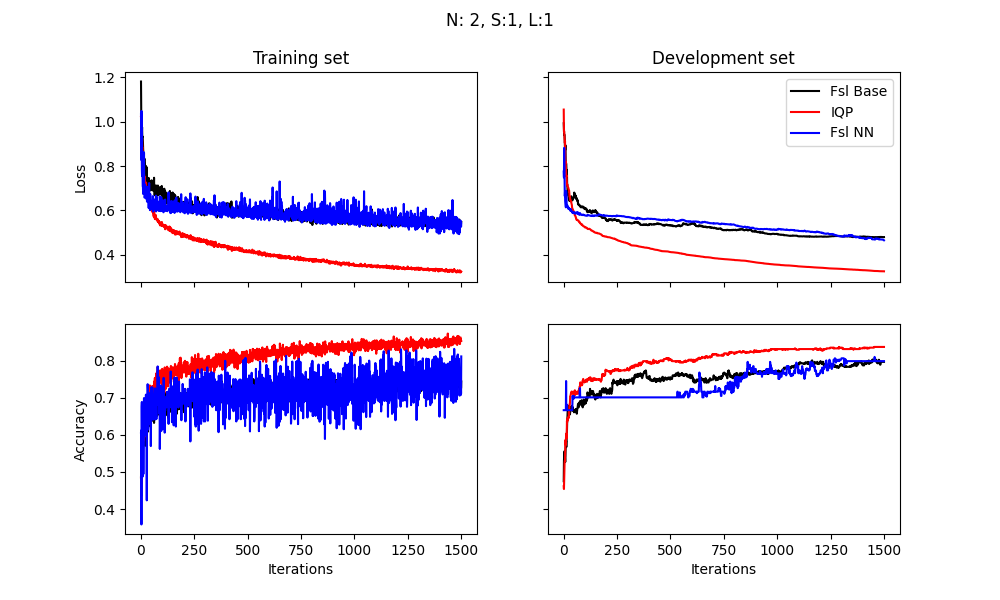
\includegraphics[width=\textwidth]{figures/comparison3/Epochs_1500--A_0.05--N_2--S_1--L_1.png}
\end{subfigure}
\begin{subfigure}[b]{.49\textwidth}
    \centering
    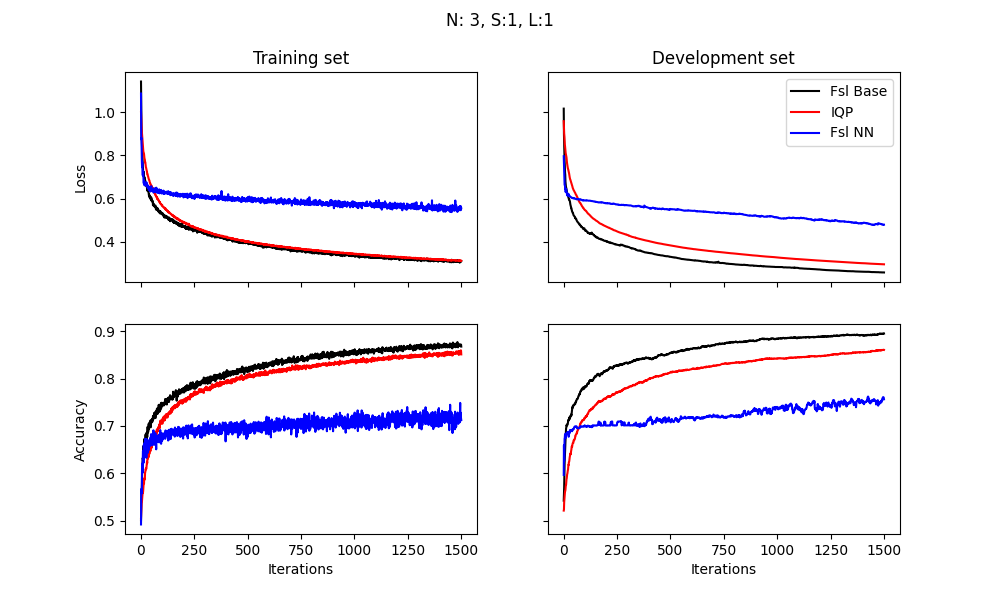
\includegraphics[width=\textwidth]{figures/comparison3/Epochs_1500--A_0.05--N_3--S_1--L_1.png}
\end{subfigure}
\begin{subfigure}[b]{.49\textwidth}
    \centering
    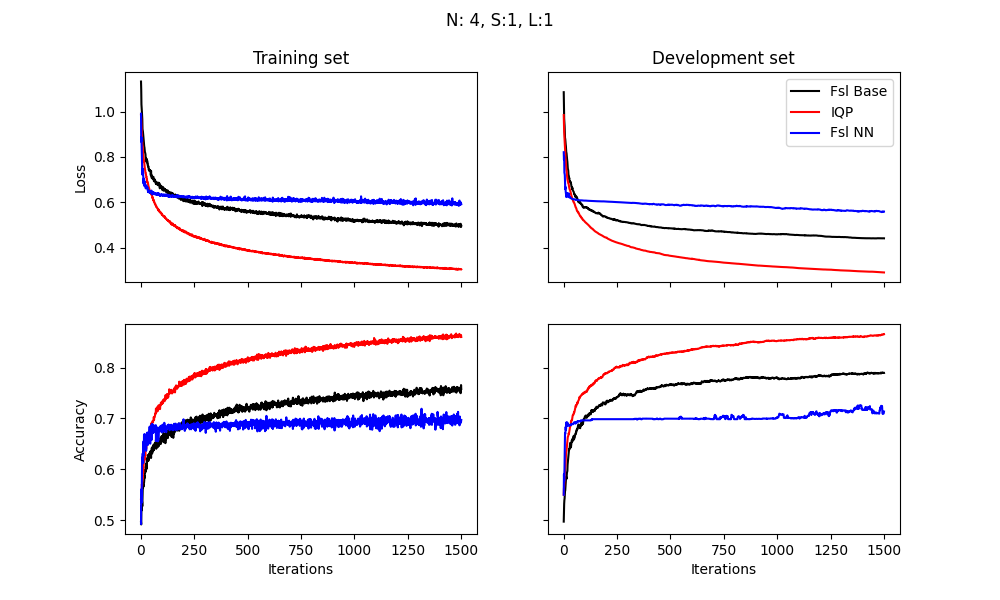
\includegraphics[width=\textwidth]{figures/comparison3/Epochs_1500--A_0.05--N_4--S_1--L_1.png}
\end{subfigure}
\caption[Comparison between three \mya for bigger datasets]{\label{fig:2spread} Training behaviour comparison between FSL NN, FSL Naive and IQP.}
\end{figure}